\section{Dominio astratto}

Nell'Esempio~\ref{example:collecting}, la computazione del least fiexed point può diventare molto costosa: gli elementi dell'insieme $M$ sono coppie di tipo $\Z \times \Z$ e il loro numero può velocemente esplodere. Cerchiamo un modo per approssimare $M$. 

\begin{definition}[Dominio]
Il \emph{dominio} è l'insieme dei valori che le variabili possono assumere all'interno dello store. 
\end{definition}

Al posto che mantenere di ogni valore il numero esatto $n \in \Z$, ne manteniamo solamente la parte di informazione che ci interessa.

\begin{example}\label{example:sign}
Il dominio dei segni è definito come segue:
\[ \set{Sign} = \{ \top, \oplus, \ominus, 0, \bot \} \]
dove $\top$ rappresenta un qualsiasi numero, $\oplus$ i numeri positivi o o nulli, $\ominus$ quelli negativi o nulli, $0$ il sono numero zero e $\bot$ nessun numero (usato come condizione d'errore, per esempio la divisione per zero). 
\end{example}

\begin{example}\label{example:interval}
Il dominio degli intervalli è definito come segue:
\[ \set{Interval} = \{ [l,h] \mid l,h \in \Z; \; l \le h \} \]
\end{example}

Entrambi i domini in Esempio~\ref{example:sign} e Esempio~\ref{example:interval} sono approssimazioni del dominio $\wp(\Z)$. I primi due prendono il nome di \emph{dominio astratto} mentre quest'ultimo è detto \emph{dominio concreto}. I domini devono formare una struttura di reticolo completo (per approfondire vedi Sezione~\ref{sec:reticoli}).

\subsection{Connessioni di Galois}\label{sec:galois-c}

Uno dei costrutti matematici che mette in relazione il dominio concreto con quello astratto è la \emph{connessione di Galois} (vedi \ref{sec:galois}). Attraverso la coppia di funzioni $\alpha, \gamma$ mappiamo gli elementi del dominio concreto in quello astratto e viceversa. 

\begin{example}
Per il dominio di Esempio~\ref{example:sign}, le funzioni $\alpha$ e $\gamma$ sono definite come segue:
\begin{align*}
    \alpha(\varnothing)                                   & = \bot                 &
    \gamma(\bot)                                          & = \varnothing          \\
    \alpha(\{0\})                                         & = 0                    &
    \gamma(0)                                             & = \{ 0 \}              \\
    \alpha(\{ x \mid \min x \ge 0 \}) & = \oplus          &
    \gamma(\oplus)                                        & = \{ x \mid x \ge 0 \} \\
    \alpha(\{ x \mid \max x \le 0 \}) & = \ominus         &
    \gamma(\ominus)                                       & = \{ x \mid x \le 0 \} \\
    \alpha(\{ x \mid \min x < 0 \land \max x > 0\})       & = \top                 &
    \gamma(\top)                                          & = \mathbb{Z}
\end{align*}
\end{example}

\begin{figure}[htbp]
    \centering
    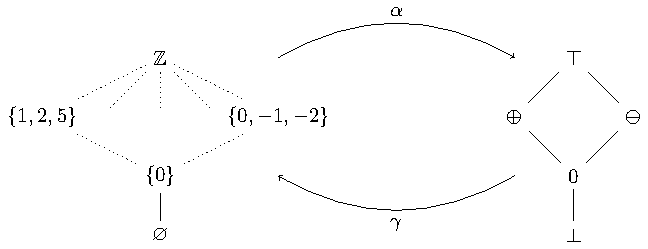
\includegraphics{capitoli/interpretazione-astratta/immagini/reticolo-segni.pdf}
    \caption{Connessione di Galois}
    \label{fig:galois-Z-sign}
\end{figure}

\subsection{Operazioni astratte}

Una volta definito il dominio astratto e la connessione di Galois, per ogni operazione $f : C \to C$ nel dominio concreto dobbiamo definire l'operazione $f^{\#} : A \to A$ nel dominio astratto. Il modo più immediato di definire $f^{\#}$ è tramite la \emph{best correct approximation}.

\begin{definition}[Best correct approximation (parzialmente preso da \cite{ranzato})]
Data una funzione $f : C \to C$ e una connessione di Galois $C \galois{\gamma}{\alpha} A$, si definisce $f^{\#} = \alpha \circ f \circ \gamma$ la \emph{best correct approximation} di $f$ in $A$.
\end{definition}

Tuttavia vorremmo poter avere il risultato di $f^{\#}$ senza dover eseguire $f$, in quanto questa potrebbe non essere calcolabile. Possiamo definire in un altro modo $f^{\#}$ e poi dimostrarne la correttezza.

\begin{definition}[Correttezza di una funzione astratta (parzialmente preso da \cite{ranzato})]
Data la connessione di Galois $C \galois{\gamma}{\alpha} A$ tra i due poset $\struct{C, \le}$ e $\struct{A, \preceq}$ ed una funzione concreta $f$, la funzione astratta $f^{\#}$ è un'approssimazione corretta di $f$ se vale
\[ \alpha \circ f = f^{\#} \circ \alpha \]
o equivalentemente
\[ f \circ \gamma = \gamma \circ f^{\#} \]
\end{definition}

\begin{example}
Consideriamo la funzione concreta $\fun{add} : \wp(\Z) \times \wp(\Z) \to \wp(Z)$:
\[ \fun{add}(X, Y) = \{ x + y \mid \forall x \in X, \, y \in Y \} \]
Per definire la sua funzione astratta nel dominio dei segni abbiamo più possibilità:
\begin{align*}
    \fun{add}^{\#}_1(s, t) 
    & = \alpha\big(\fun{add}(\gamma(s), \gamma(t)) \big) \\[1em]
    \fun{add}^{\#}_2(s,t) 
    & = \begin{array}{c c c c c c}
             & \multicolumn{5}{c}{t}                       \\\cmidrule{2-6}
    s        & \top   & \oplus & \ominus & 0       & \bot  \\\midrule
    \top     & \top   & \top   & \top    & \top    & \bot  \\
    \oplus   & \top   & \oplus & \top    & \oplus  & \bot  \\
    \ominus  & \top   & \top   & \ominus & \ominus & \bot  \\
    0        & \top   & \oplus & \ominus & 0       & \bot  \\
    \bot     & \bot   & \bot   & \bot    & \bot    & \bot  \\
\end{array} \\[1em]
    \fun{add}^{\#}_3(s,t) 
    & = \top
\end{align*}
Tutte e tre le varianti sono corrette. 
\end{example}

